\label{addtools}

\section{Additional Tools}
For a further investigation of the static performances, it is possible to use additional tools. These can be selected by clicking on Tools, in the upper part of the CSAtool window.

\begin{description}

	\item[PPEX Tool] \hfill \\
	In case the extracted values of the parasitic capacitances are available from a post-layout analysis and/or if the user desired to investigate the effects produced by  localized parasitics, PPEX tool allows to add the value of the parasitic capacitance connected from the top plate to the bottom plate of each capacitive bank in the array. This is possible through the dedicated user interface shown in figure \ref{fig:ppex}. 

\begin{itemize}
\item Which is the difference between PPEX tool and the modules dedicated to \texttt{Specific Parasitics} and  \texttt{External Parasitics} that are already provided in CSAtool main window?
\end{itemize}

The external parasitics are just those connected from the top-plate of each eventual sub-DAC and the reference nets (substrate, VDD, GND ...).The specific parasitics are top-to-substrate (or reference nets), top-to-bottom, and bottom-to-substrate (or reference nets) stray capacitances that affect in general each unit capacitor, thus also the capacitive banks since each of them is built by multiple unit capacitors. These capacitances are specific so they depend on the area of the unit capacitor and so of each bank; in general they are proportional to the capacitance. 
PPEXtool offers the chance to estimate the effect of all those parasitics connected from the top to the bottom of any of the capacitive banks, which are not directly dependent on the area but on other issues, for example the layout quality, which depends only on the designer ability. This can be the case of wiring parasitics. 
Once a parasitic set is loaded and applied, all the analysis available from CSAtool can be performed through the main window and the other modules.
It is worth noting here that \textbf{the parasitic loaded through PPEXtool sum to the others specified in the main window} and also to the mismatch effect. 

\begin{figure}[h!]
	\centering
	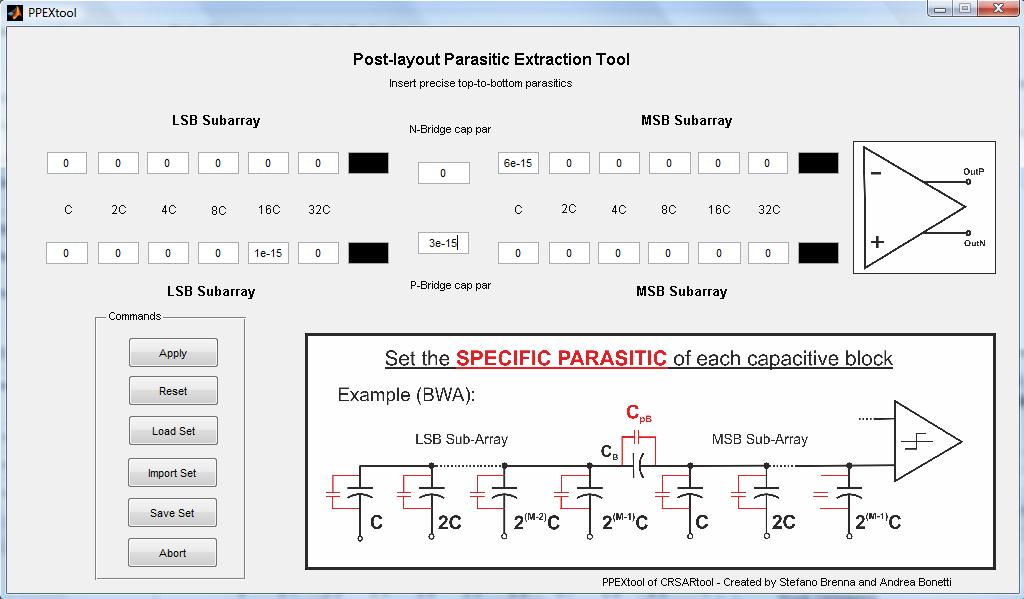
\includegraphics[scale=0.35]{pics/ppex.jpg}
	\caption{PPEX module for a 12-bit fully differential BWA.}
	\label{fig:ppex}
\end{figure}

	\item[SSA Tool] \hfill \\
	This tool provides a statistical analysis of the static performance over a desired number of runs, set by the parameter \texttt{Runs}. The parameter \texttt{sigma} act as a multiplier for the currently set pelgrom mismatch coefficient $k_{c}$. SSA tool output is represented by the standard deviation of DNL and INL as a function of the output code and by the distribution of their maximum absolute value.
\begin{figure}[h!]
	\centering
	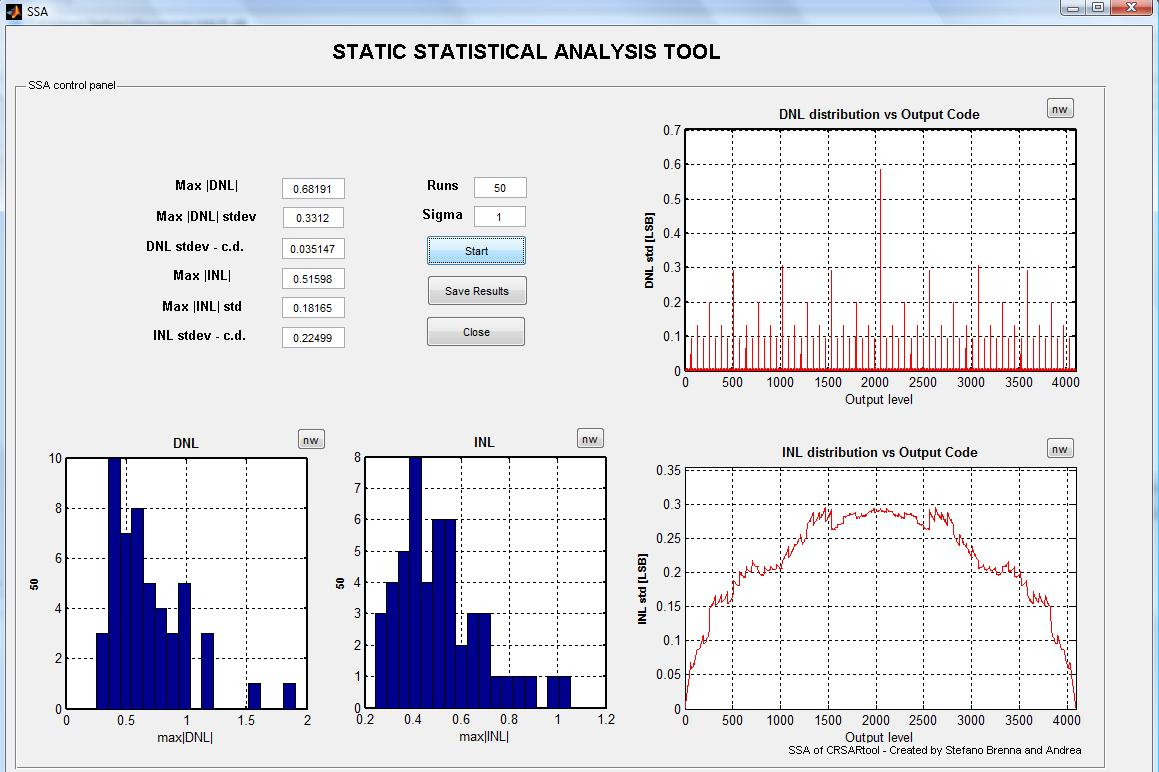
\includegraphics[scale=0.35]{pics/ssa.jpg}
	\caption{Static Statistical Analysis module.}
	\label{fig:ppex}
\end{figure}

	\item[ESA Tool] \hfill \\
	A statistical analysis of the achievable ENoB is presented here. The working principle is the same of SSAtool. The maximum ENoB distribution is evaluated over a desired number of runs, set by the parameter \texttt{Runs}. For each realization, the input amplitude of a virtual input sinusoid spans between the given minimum and maximum amplitudes, set by the users as a fraction of the FSR by defining the parameters \texttt{Minimum Input} and  \texttt{Minimum Input}.

\begin{figure}[h!]
	\centering
	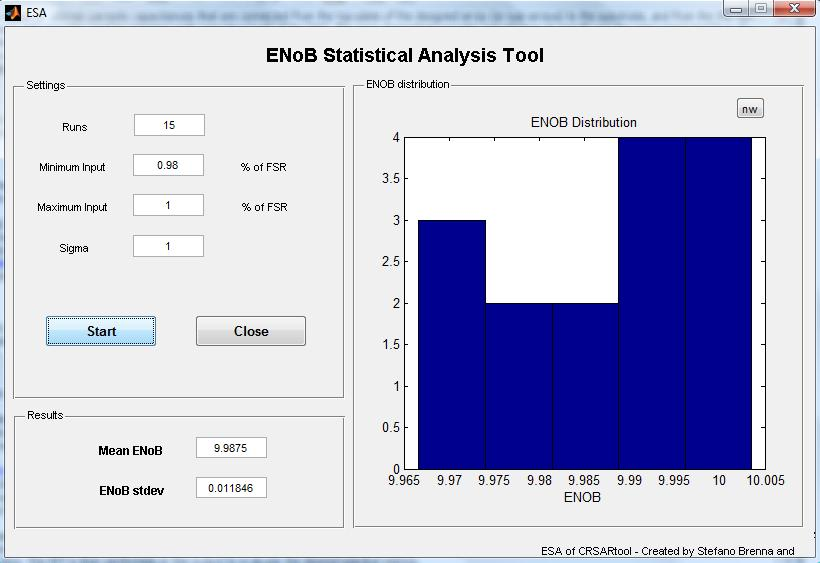
\includegraphics[scale=0.5]{pics/ESA.jpg}
	\caption{ESA module GUI.}
	\label{fig:esa}
\end{figure}



\end{description}